\documentclass[a4paper,11pt,titlepage]{article}
% The maths package
\usepackage{amsmath}
\usepackage{amsfonts}
% The graphics package
\usepackage{graphicx}
% Allows paragraph in blocks
\usepackage{parskip}
% Code hightling
\usepackage{minted}
% Verbatim file inclusion
\usepackage{fancyvrb}
% For loops
\usepackage{pgf,pgffor}
% For placing figures
\usepackage{float}

%%%% Define the title %%%%%%%%%%%%%%%%%%%%%%%%%%%%%%%%%%%%%%%%%%%%%%%%%%%%%%%%%%
\title{
MECH3750 Engineering Analysis II \\ 
Assignment 2
}
% define the author
\author{
Merrick Heley\\
42339915
}

%%%% Notes, commands, settings %%%%%%%%%%%%%%%%%%%%%%%%%%%%%%%%%%%%%%%%%%%%%%%%%
% \section*{Task 1} uses an asterisk to suppress the section number

% This command adds \ud for finishing integrals
\newcommand{\ud}{\,\mathrm{d}}

% Set the pygmentation style for code
% pygmentize -L styles
\usemintedstyle{autumn}

% Simple command for python file input
\newcommand{\inputpython}[1]{
    \inputminted[linenos=true, 
                 frame=single, 
                 fontsize=\scriptsize, 
                 label=#1]
                {python}{#1}
}

% Simple command for python file output
\newcommand{\pythonoutput}[1]{
    \immediate\write18{python #1 > #1.out}
    \fvset{frame=single, numbers=left, fontsize=\scriptsize, label=#1.out}
    \VerbatimInput{#1.out}
    \write18{del #1.out}
}

% Simple command for python file input
\newcommand{\inputmaxima}[1]{
    \inputminted[linenos=true, 
                 frame=single, 
                 fontsize=\scriptsize, 
                 label=#1]
                {cpp}{#1}
}

%%%% Start document %%%%%%%%%%%%%%%%%%%%%%%%%%%%%%%%%%%%%%%%%%%%%%%%%%%%%%%%%%%%

\begin{document}
% generates the title
\maketitle

%%%% Question 0.1 %%%%%%%%%%%%%%%%%%%%%%%%%%%%%%%%%%%%%%%%%%%%%%%%%%%%%%%%%%%%%%
\section*{Question 0.1: Boundary Value Problems}
\subsection*{a. Shooting Method}

\begin{align}
-y'''(x) + y''(x) - 4xy'(x) + (8x + 3)y(x) &= x^2 \label{eq:q1bvp}\\
y(-1) & = -10 \notag\\
y(0.5) & = 1 \notag\\
y(1.5) & = -3 \notag
\end{align}

The first step to solving this problem is to rearrange the equation for $y'''$

\begin{equation}
y''' = (1)y'' + (-4x)y' + (8x + 3)y - x^2
\end{equation}

The equation can then be put into matrix form
\begin{equation}
\begin{bmatrix}
y' \\
y'' \\
y'''
\end{bmatrix}
=
\begin{bmatrix}
    0       &   1       &   0 \\
    0       &   0       &   1 \\
    8x+3    &   -4x     &   1
\end{bmatrix}
\begin{bmatrix}
y \\
y' \\
y''
\end{bmatrix}
+
\begin{bmatrix}
0 \\
0 \\
-x^2
\end{bmatrix}\label{eq:rk4mat}
\end{equation}
Also expressed as
\begin{equation}
F(x, Y) = Z(x)Y + C(x) \label{eq:rk4func}
\end{equation}

which is compatible with a Runge-Kutta 4 (RK4) ODE solver.

Runge-Kutta 4 is an iterative ODE solver of the form:
\begin{align}
k_1 & = F(x_i, Y_i) \notag\\
k_2 & = F(x_i + 0.5h, Y_i + 0.5*h*k1) \notag\\
k_3 & = F(x_i + 0.5h, Y_i + 0.5*h*k2) \notag\\
k_4 & = F(x_i + h, Y_i + h*k3) \notag\\
Y_{i+1} & = Y_i + \frac{1}{6}\left(k_1 + 2k_2 + 2k_3 + k_4\right) \notag
\end{align}
which allows for the next Y value to be generated from the current Y value
(the initial values), the x value and the step size.

In this case, the initial values are the values for $y$, $y'$ and $y''$ 
which are given for the Y matrix as shown in 
\eqref{eq:rk4mat}, and the function \eqref{eq:rk4func} is passed to the RK4 
solver as the ODE equation.

Shooting method operates by letting the user take a guess at the initial values 
for the solution, and then compare it with the known boundary values, 
essentially implementing a 'guess and check' approach.

To check the correctness of the guess, the values obtained by using RK4 solver 
have been recorded at each step and plotted against the boundary values. 
Various guesses have been included, as seen in line 109, ``\# Array of guesses''.

\inputpython{Task1a.py}
\pythonoutput{Task1a.py}

\foreach \x [count=\xi] in {0,...,7} {%
    \begin{figure}[H]
    \centering
    \includegraphics[scale=0.5]{Guess\x.png}
    \caption{Solution to BVP from guess \xi}
    \end{figure}
}

\subsection*{b. Lehmer-Shur Algorithm}

The Lehmer-Shur algorithm is an extension to the bisection method that 
expands it to a two dimensional root finder. This can be used to find the roots 
of the BVP by forming a rectangle around the solution, then performing 
bisection in both dimensions to reduce the size of the rectangle until a root 
is found.

However, the bisection method only converges linearly. The efficiency of the 
Lehmer-Shur algorithm an therefore be improved by using a two dimension 
secant method, which converges super-linearly.

To implement this, a secant method has been written (see Appendix A). This 
top level secant method guesses a value for $y''$ and calls the findydd 
function. The findydd function then calls another secant method, which 
guesses a value for $y'$ and calls the function findyd. 

The findyd treats $y''$ as a constant, and the secant method finds a value for 
$y'$ that satisfies the first boundary value. This value for $y'$ is then 
passed up to the findydd function, which checks if the solution satisfies 
the second boundary condition. If it does, the secant method has found a 
solution to the BVP, if not the process is repeated for a refined guess 
of $y''$.

\inputpython{Task1b.py}
\pythonoutput{Task1b.py}

\begin{figure}[H]
\centering
\includegraphics[scale=0.5]{Task1b.png}
\caption{Solution to BVP using Shooting Method with Secant}
\end{figure}

\subsection*{c. Difference Method}

To solve this boundary value problem using difference method, approximations 
must be formed using a difference approximation. To keep the problem simple, a 
first order central difference method was initially used.

\begin{align}
y' & = \frac{1}{2h}(y_{i+1} - y_{i-1}) \label{eq:central1}\\
\intertext{When this equation is substituted into itself, it can be derived 
            further}
y'' & = \frac{1}{h^2}(y_{i+1} - 2y_i + y_{i-1}) \label{eq:central2}\\
\intertext{And once more}
y''' & = \frac{1}{2h^3}(y_{i+2} - 2y_{i+1} + 2y_{i-1} - y_{i-2}) 
            \label{eq:central3}
\intertext{Substituting \eqref{eq:central1} \eqref{eq:central2} \eqref{eq:central3} 
            into \eqref{eq:q1bvp}}
x_i^2 & = -\frac{1}{2h^3}(y_{i+2} - 2y_{i+1} + 2y_{i-1} - y_{i-2}) \notag\\
      &   + \frac{1}{h^2}(y_{i+1} - 2y_i + y_{i-1}) \notag\\
      &   - \frac{4x}{2h}(y_{i+1} - y_{i-1}) \notag\\
      &   + (8x + 3)y_i \\
\intertext{And rearranging to group $y_i$ values together}
x_i^2 & = \left(\frac{1}{2h^3}\right)y_{i-2} + \notag\\
      & \left(\frac{-2}{2h^3} + \frac{1}{h^2} + \frac{4x}{2h}\right)y_{i-1} + \notag\\
      & \left(\frac{-2}{h^2} + (8x + 3)\right)y_i + \notag\\
      & \left(\frac{2}{2h^3} + \frac{1}{h^2} + \frac{-4x}{2h}\right)y_{i+1} + \notag\\
      & \left(\frac{-1}{2h^3}\right)y_{i+2} \label{eq:bvpcentral} \\
\intertext{This equation is modelled in the function 'f(x, h)' in the code}
\intertext{It can be seen in \eqref{eq:bvpcentral} that at the first and final
            steps, an invalid value will be referenced (e.g. at -0.9, $y_{i-2}$
            will correspond to -1.1, at which we have no data). To handle this,
            \eqref{eq:central2} will be derived using a forward difference 
            method rather than a central difference method.}
\intertext{The forwards difference approximation is}
y' & = \frac{1}{h}(y_{i+1} - y_i) \label{eq:forward1}\\
\intertext{And deriving \eqref{eq:central2} with \eqref{eq:forward1} gives}
y''' & = \frac{1}{h^3}(y_{i+2} - 3y_{i+1} + y_i - y_{i_1}) \label{eq:forward3}\\
\intertext{Substituting \eqref{eq:central1} \eqref{eq:central2} \eqref{eq:forward3}
            in to \eqref{eq:q1bvp} and rearranging to group $y_i$ values together}
x_i^2 & = \left(0\right)y_{i-2} + \notag\\
      & \left(\frac{1}{h^3} + \frac{1}{h^2} + \frac{4x}{2h}\right)y_{i-1} + \notag\\
      & \left(\frac{-3}{h^3} + \frac{-2}{h^2} + (8x + 3)\right)y_i + \notag\\
      & \left(\frac{3}{h^3} + \frac{1}{h^2} + \frac{-4x}{2h}\right)y_{i+1} + \notag\\
      & \left(\frac{-1}{h^3}\right)y_{i+2} \label{eq:bvpforward}\\
\intertext{This equation is modelled in the function 'fForward(x, h)' in the code}
\intertext{Using the backwards difference approximation}
y' & = \frac{1}{h}(y_{i} - y_{i-1}) \label{eq:backward1}\\
\intertext{and a similar process to the forward difference method, the final 
            grouped $y_i$ values with the backwards difference method subbed 
            in are}
x_i^2 & = \left(\frac{1}{h^3}\right)y_{i-2} + \notag\\
      & \left(\frac{-3}{h^3} + \frac{1}{h^2} + \frac{4x}{2h}\right)y_{i-1} + \notag\\
      & \left(\frac{3}{h^3} + \frac{-2}{h^2} + (8x + 3)\right)y_i + \notag\\
      & \left(\frac{-1}{h^3} + \frac{1}{h^2} + \frac{-4x}{2h}\right)y_{i+1} + \notag\\
      & \left(0\right)y_{i+2} \label{eq:bvpbackward}
\intertext{This equation is modelled in the function 'fBackward(x, h)' in the code}\notag
\end{align}
To generate a solution to this equation, it is necessary to solve the equation
\begin{equation}
JY = X
\end{equation}
Where $J$ is the $n \times n$ system of equations for the LHS of the system, 
$X$ is the $n \times 1$ matrix of the RHS of the system
and $Y$ is the set of $y$ values at each point on $X$.

As the step size is known (at 0.1) a 26x26 matrix can be made (the code is 
invariant to this step size, however significantly increasing it will slow 
the execution time) and can be populated along its diagonal using the central 
difference method. In cases where the central difference method will attempt to 
use values outside the matrix (i.e. close to the edges of the matrix), forwards 
and backwards difference methods can be used (see line 155 ``\# Handle difference 
approximation at boundaries'' in the code

Finally, at x values where the solution is known (i.e. the boundary values), 
the element in the $X$ matrix corresponding to this point should be set to the 
known solution (see line 57 ``\# Handle boundary values'' in the code) and the 
corresponding row in the $J$ matrix should be set to all 0's with a single '1'
in it's diagonal element (see line 82 ``\# Handle boundary values'' in the code).

These generated matrices are shown in the output of the python code.

\inputpython{Task1c.py}
\pythonoutput{Task1c.py}

\begin{figure}[H]
\centering
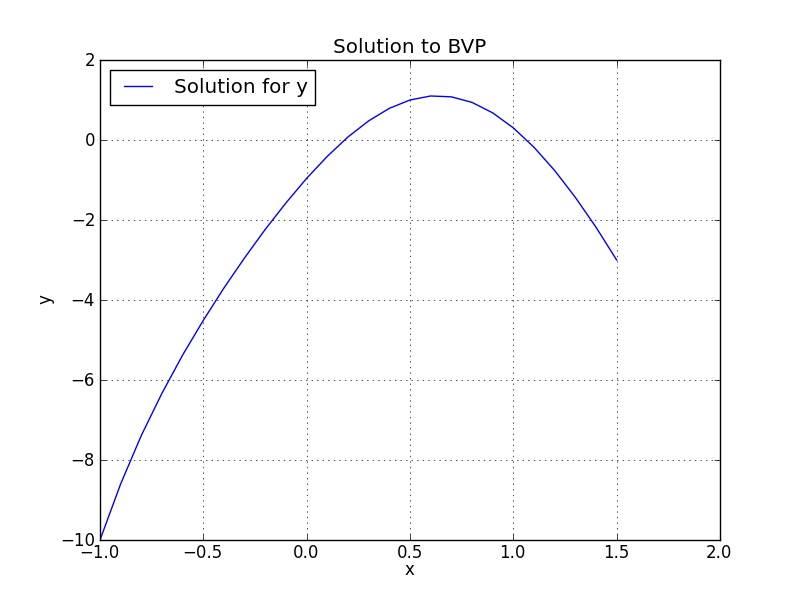
\includegraphics[scale=0.5]{Task1c.png}
\caption{Solution to BVP using Difference Method}
\end{figure}

It can be seen the solution using the difference method is extremely similar to 
the solution using the shooting method.

\subsection*{d. Non-Linear Difference Method}

\begin{align}
y''(x) + (cos(y(x)) + 2)^2 - 9x^3y(x)^2 & = 0 \\
y(1) & = 1  = BV(0) \notag\\
y(1.8) & = 3 = BV(1) \notag
\end{align}
The first step to solving this ODE is applying a second order central 
difference method to $y''$ such as \eqref{eq:central2}.
\begin{equation}
0 = \frac{1}{h^2}(y_{i+1} - 2y_i + y_{i-1}) + (cos(y_i) + 2)^2 - 
9x_i^3y_i^2 \notag
\end{equation}

There will need to be an equation for step of the solution. For an equation with
n steps (e.g. for h=0.1, $\frac{1.8 - 1}{0.1} - 1 = 7$ steps):

\begin{align}
0 & = \frac{1}{h^2}(y_1 - 2y_0 + BV(0) ) + (cos(y_0) + 2)^2 - 9x_0^3y_0^2 \notag\\
0 & = \frac{1}{h^2}(y_2 - 2y_1 + y_0 ) + (cos(y_1) + 2)^2 - 9x_1^3y_1^2 \notag\\
...\notag\\
0 & = \frac{1}{h^2}(y_n - 2y_{n-1} + y_{n-2} ) + (cos(y_{n-1}) + 2)^2 - 9x_{n-1}^3y_{n-1}^2 \notag\\
0 & = \frac{1}{h^2}(BV(1) - 2y_n + y_{n-1} ) + (cos(y_n) + 2)^2 - 9x_n^3y_n^2 \notag
\end{align}

Due to the similarity of the functions, an entire list can be generated from a 
single generic function, as implemented in the code in genFunctionList.

This method gives a system of equations with N equations and N unknowns, 
which is solvable using a multi-dimensional newtons method. This is discussed 
in detail in Question 0.2: Newtons Method.

\inputpython{Task1d.py}
\pythonoutput{Task1d.py}

\begin{figure}[H]
\centering
\includegraphics[scale=0.5]{Task1d.png}
\caption{Solution to BVP using Difference Method}
\end{figure}

%%%% Question 0.2 %%%%%%%%%%%%%%%%%%%%%%%%%%%%%%%%%%%%%%%%%%%%%%%%%%%%%%%%%%%%%%
\section*{Question 0.2: Newtons Method}
\subsection*{a. Single Solution}

\begin{align}
x^3 + 3x^2y - 2xy^2 - 7y^3 & = -604894015496000 \label{eq:newt1}\\
-15x^2 - 57xy - 67y^2 & = -26864190700 \label{eq:newt2}
\end{align}

This is a system of equations with two equations and two unknowns. As such, it 
is solvable using a multi-dimensional Newtons method. Multidimensional Newtons 
method is an application of the truncated Taylor series

\begin{equation}
x_1 = x_0 - \frac{f(x_0)}{f'(x_0)} \notag
\end{equation}

that is expanded for a system of equations and repeated until the change 
falls below a threshold. When expanding this system, as there are multiple 
variables, partial derivatives must be used for each equation.

\begin{equation}
F(x,y,...) \approx
\begin{bmatrix}
f_1 (P_0) \\
f_1 (P_0) \\
\vdots
\end{bmatrix}
+
\begin{bmatrix}
    \frac{\partial}{\partial x} f_1 (P_0) & \frac{\partial}{\partial y} f_1 (P_0) &   \ldots \\
    \frac{\partial}{\partial x} f_2 (P_0) & \frac{\partial}{\partial y} f_2 (P_0) &   \ldots \\
    \vdots    &   \vdots     &   \ddots
\end{bmatrix}
.
\begin{bmatrix}
x - x_0 \\
y - y_0 \\
\vdots
\end{bmatrix}
\end{equation}

Which can be iterated over until the matrices reach equilibrium (i.e. the 
change in the matrix falls below a threshold) after an initial guess is given.

To solve this particular system of equations, only a 2 variable system is needed.
However, a general solution (as has been implemented below), will generate the 
system based on the number of equations given to it. The can be used to solve 
not only this system of equations, but other systems of equations (and is used 
to solve Task 1d).

\inputpython{Newtons.py}

It was found for this system of equations that real guesses for the system 
would not find equilibrium, i.e. the system had no real solutions 
(which can be verified by plotting the equations). As such, 
a complex guess was used to find a complex solution.

\begin{figure}[H]
\centering
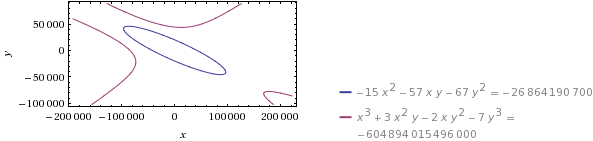
\includegraphics[scale=0.8]{Task2aplot.png}
\caption{Plot of \eqref{eq:newt1} \eqref{eq:newt2} in $\mathbb{R}$}
\end{figure}

\inputpython{Task2a.py}
\pythonoutput{Task2a.py}

\subsection*{b. Solutions in $\mathbb{C}$}

As the system can be observed to have approximately 6 solutions, with 
3 unique sets of values and 3 complex conjugates, complex conjugate guesses 
were used (shown in c. Proof of number of solutions).

As such, complex conjugate initial guesses were used that had an increasingly 
large absolute value were used. The guesses that gave unique solutions were 
included below.

If no information about the nature of the solutions could be deduced (such as 
the solutions would be complex conjugates of each other), a brute-force method 
for a sample of complex values in a range should be used (similar to d. Maxima 
Brute-force), and unique solutions should be recorded.

\inputpython{Task2b.py}
\pythonoutput{Task2b.py}

\subsection*{c. Proof of number of solutions}

Matlab was used to rearrange \eqref{eq:newt2} and sub it in to \eqref{eq:newt1} 
using matlab.

It was found that when \eqref{eq:newt2} was rearranged, it was split into 
two equations (as it is a formula for an ellipse, $y = \pm F(x)$). Substituting 
this back into \eqref{eq:newt1} and simplifying gives a cubic for both 
rearrangements of \eqref{eq:newt2}.

This gives two cubics as final solutions, with 3 roots each (6 roots in total).
As it has been observed in 2a. that there are no real solutions, and the
rearrangement of \eqref{eq:newt2} gave a $\pm F(x)$, it is reasonable to assume 
these solutions are complex conjugates.

\begin{minted}[linenos=true, 
               frame=single, 
               fontsize=\scriptsize, 
               label=Task2c Matlab Command Line]
               {matlab}
>> solve('-15*x^2 - 57*x*y - 67*y^2 = -26864190700', 'y')
ans =
   (7199603107600 - 771*x^2)^(1/2)/134 - (57*x)/134
 - (57*x)/134 - (7199603107600 - 771*x^2)^(1/2)/134
>> y =  (7199603107600 - 771*x^2)^(1/2)/134 - (57*x)/134;
>> S = x^3 + 3*y*x^2 - 2*x*y^2 - 7*y^3;
>> pretty(simplify(S))
 
                                                       2 1/2 
  12478416580150 x   94024667450 (7199603107600 - 771 x )    
  ---------------- - --------------------------------------- 
        4489                          4489                   
        
                  2                       2 1/2           3 
            5397 x  (7199603107600 - 771 x )      238753 x       
        + ----------------------------------- - ---------   
                         601526                   601526
>> y = - (57*x)/134 - (7199603107600 - 771*x^2)^(1/2)/134;
>> S2 = x^3 + 3*y*x^2 - 2*x*y^2 - 7*y^3;
>> pretty(simplify(S2))
 
                                                       2 1/2 
  12478416580150 x   94024667450 (7199603107600 - 771 x )    
  ---------------- + --------------------------------------- 
        4489                          4489                   
        
                  2                       2 1/2           3 
            5397 x  (7199603107600 - 771 x )      238753 x       
        - ----------------------------------- - ---------   
                         601526                   601526
\end{minted}

\subsection*{d. Maxima Brute-force}

To verify there are no real, whole number solutions, Maxima code was written 
that guesses every value of x and y in a very large range and checks if this 
solves the equations. This would take an extremely long time to run, and 
would yield no results.

\inputmaxima{Task2d.wxm}

%%%% APPENDICES %%%%%%%%%%%%%%%%%%%%%%%%%%%%%%%%%%%%%%%%%%%%%%%%%%%%%%%%%%%%%%%%
\clearpage
\section*{Appendix A}
% Secant method in appendix (shitty, and not correct way of doing appendices)
\inputpython{secant.py}
\pythonoutput{secant.py}

\clearpage
\end{document}